\documentclass[12pt]{article}
\usepackage{amsmath, amssymb}
\usepackage{pdfpages}
\usepackage[a4paper, top=18mm, bottom=18mm, left=10mm, right=10mm]{geometry}
\usepackage[font = normalsize, labelfont = bf]{caption}
\usepackage[font = normalsize, labelfont = bf]{subcaption}
\usepackage{epsf, graphics}
\usepackage[toc,page]{appendix}
\usepackage{tcolorbox}
\usepackage{fancyhdr}
\usepackage{lipsum, lastpage}
\usepackage[official]{eurosym}
\usepackage{colortbl, tabularx}
\usepackage{color, enumerate, natbib}
\usepackage{hyperref}  % this guy must be the last package called
\hypersetup{colorlinks=true, allcolors=blue}


\begin{document}

\pagestyle{fancy}
\lhead{\footnotesize \parbox{11cm}{MHD Workshop Leiden 2021}}
\rhead{\footnotesize \parbox{11cm}{\hfill \textsf{Legolas} demo}}
\renewcommand\headheight{24pt}
\renewcommand\footrulewidth{0.4pt}

\section*{Getting started}
The Legolas code can be found on \href{https://github.com/n-claes/legolas}{GitHub}, installation instructions are on the website. Make sure to look at the prerequisites for both Legolas and Pylbo first before running the code.

\section{Equilibria}
Below is a list of possible setups that can be implemented in the user submodule. We've added a reference figure together with the link to the original work so you can check your implementation and compare with known results.

\subsection{Internal kink modes in force-free magnetic fields}
This setup is taken from \citet{goedbloed2018} and corresponds to a cylindrical equilibrium with a force-free magnetic field of constant $\alpha$ and profiles given by
\begin{equation*}
	\begin{aligned}[t]
		\rho(r) &= \rho_0\left(1 - x^2\right) \\
		v_z(r) &= v_{03}\left(1 - x^2\right) \\
		B_\theta(r) &= J_1(\alpha x) \\
		B_z(r) &= J_0(\alpha x) \\
		T(r) &= \frac{p_0}{\rho(r)}
	\end{aligned}
	\qquad\qquad
	\begin{aligned}[t]
		\rho'(r) &= -\frac{2\rho_0}{a} x \\
		v_z'(r) &= -\frac{2v_{03}}{a} x \\
		B_\theta'(r) &= \frac{\alpha}{2a} \left[J_0(\alpha x) - J_2(\alpha x)\right] \\
		B_z'(r) &= -\frac{\alpha}{a} J_1(\alpha x) \\
		T'(r) &= \frac{2 r p_0}{a^2\rho_0(1 - x^2)^2}
	\end{aligned}
\end{equation*}
where $x = r / a$ and $a$ denotes the outer wall of the cylinder.

\begin{figure}[h]
	\centering
	\begin{minipage}{0.42\textwidth}
		\centering
		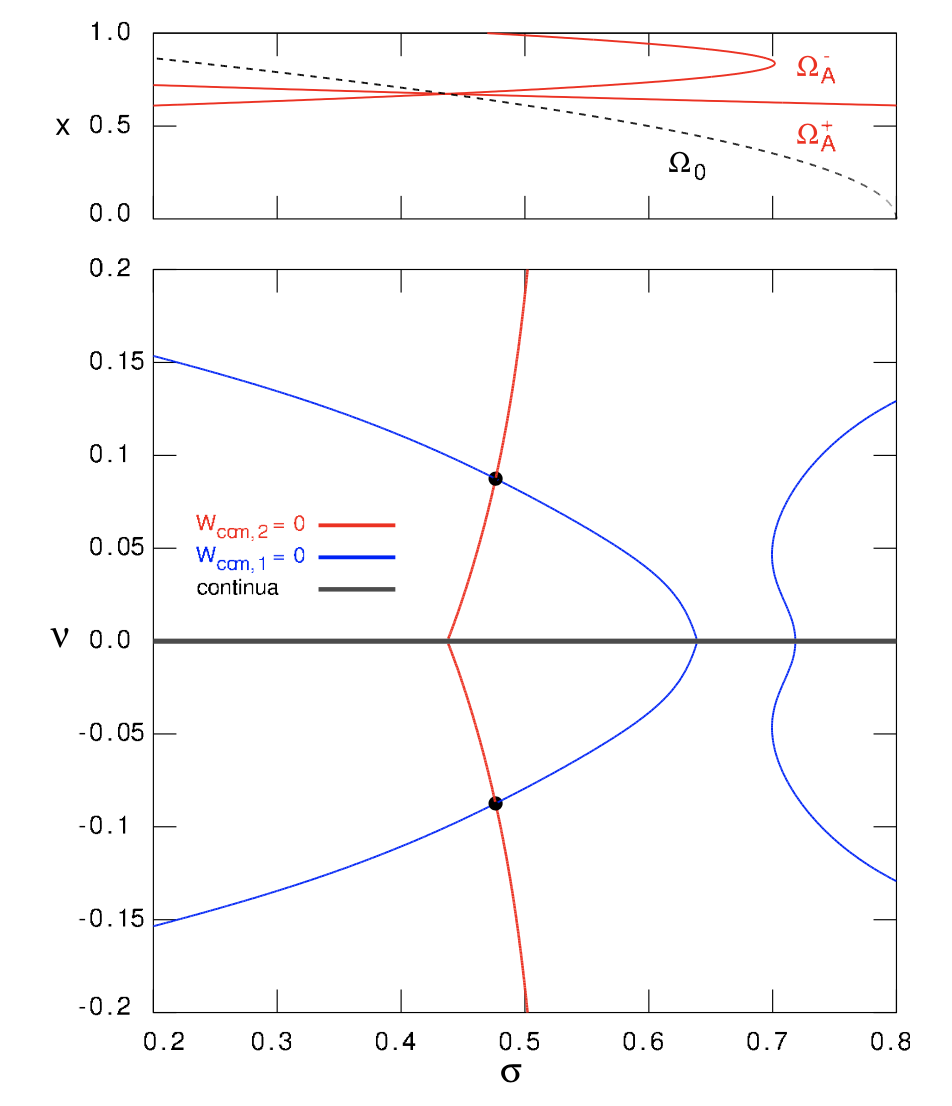
\includegraphics[width=\textwidth]{internal_kink.png}
		\caption{Values $\rho_0 = v_{03} = p_0 = a = m = 1$, $\alpha a = 5$, $k = 0.16\alpha$, incompressible.}
	\end{minipage}\hfill
	\begin{minipage}{0.53\textwidth}
		\centering
		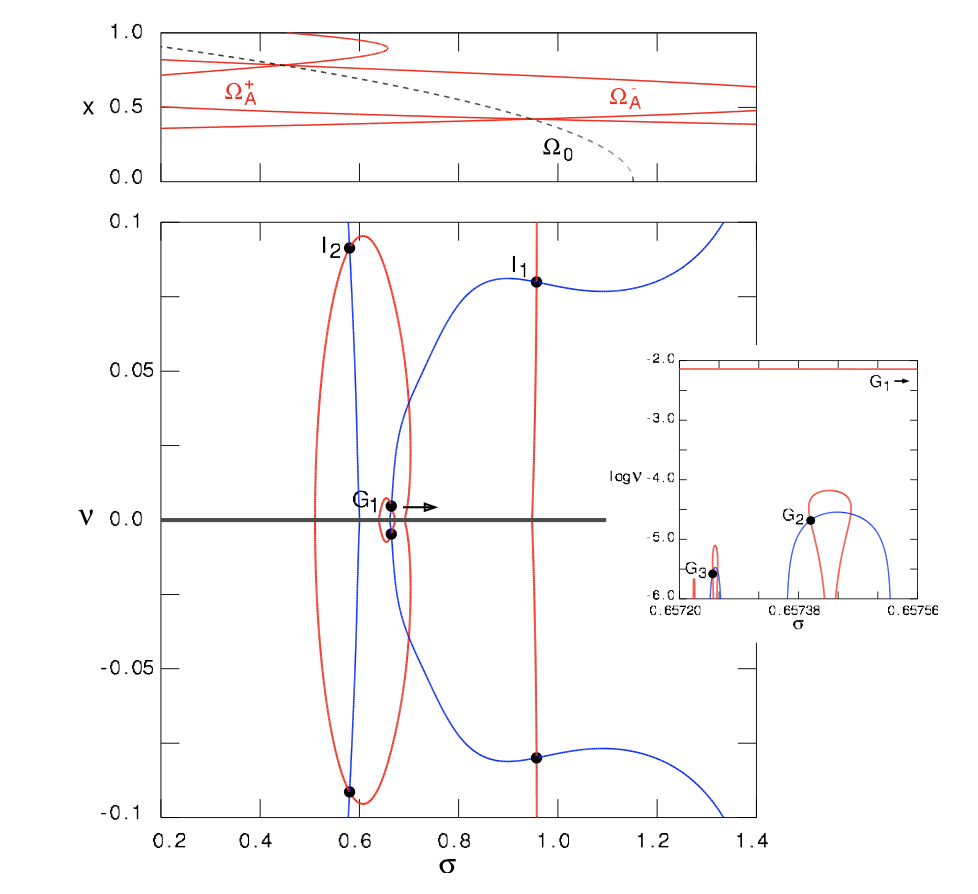
\includegraphics[width=\textwidth]{internal_kink2.png}
		\caption{Values $\rho_0 = p_0 = a = m = 1$, $v_{03} = 0.8$, $\alpha a = 8$, $k = 0.16\alpha$, incompressible.}
	\end{minipage}
\end{figure}

\subsection{RTI in rotating theta-pinches}
This setup is taken from \citet{goedbloed2018} and corresponds to Rayleigh-Taylor instabilities in rotating theta-pinches.
Introducing the following quantities
\[ x = \frac{r}{a} \qquad\qquad f_x = \alpha^2\left(x^2 - r_0^2\right) \qquad\qquad f_x' = \frac{2\alpha^2 x}{a} \]
where $a$ denotes the cylinder wall and $r_0 = 0$ in this case.
The equilibrium is then given by
\begin{equation*}
	\begin{aligned}[t]
		\rho(r) &= \frac{\rho_0}{\cosh^2(f_x)} \\
		v_\theta(r) &= \Omega r \\
		B_z(r) &= B_\infty\left[\delta + \left(1 - \delta\right)\tanh(f_x)\right] \\
		T(r) &= \frac{p_0}{\rho_0} \\
	\end{aligned}
	\qquad\qquad
	\begin{aligned}[t]
		\rho'(r) &= \frac{-2\rho_0 f_x' \tanh(f_x)}{\cosh^2(f_x)} \\
		v_\theta'(r) &= \Omega \\
		B_z'(r) &= \frac{B_\infty\left(1 - \delta\right)f_x'}{\cosh^2(f_x)}
	\end{aligned}
\end{equation*}
where
\[ p_0 = \frac{1}{2}\left(1 - \delta\right)^2, \qquad B_\infty = a\sqrt{\rho_0}, \qquad \Omega = \alpha \sqrt{2\delta(1 - \delta)}\]

\begin{figure}[h]
	\centering
	\begin{minipage}{0.50\textwidth}
		\centering
		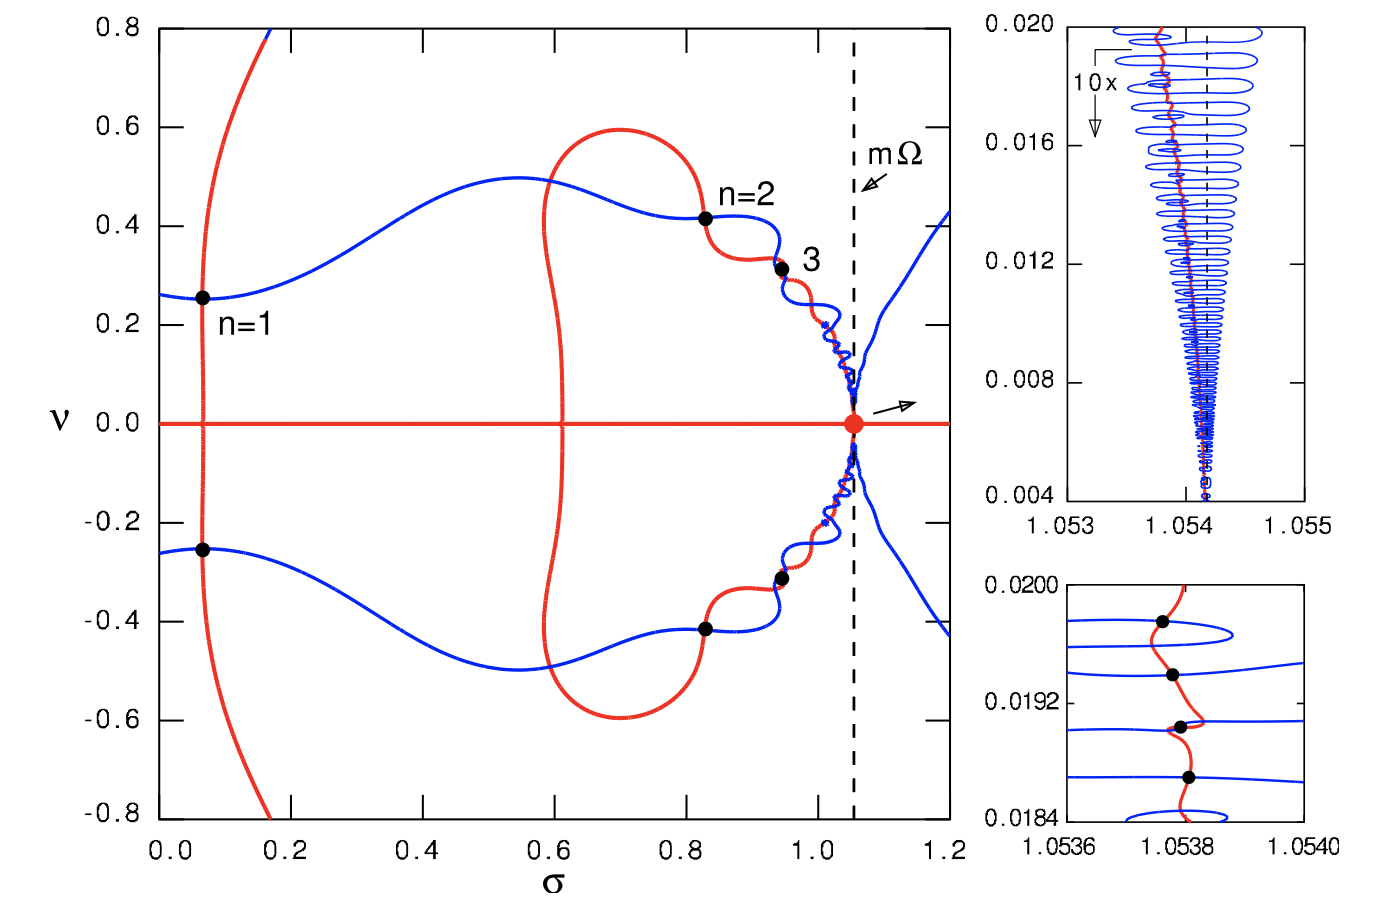
\includegraphics[width=\textwidth]{RTI_HD.png}
		\caption{Values $\rho_0 = a = m = 1$, $\alpha = 2$, $\delta = 1/6$, $k = 0$ (hydrodynamics), incompressible.}
	\end{minipage}\hfill
	\begin{minipage}{0.45\textwidth}
		\centering
	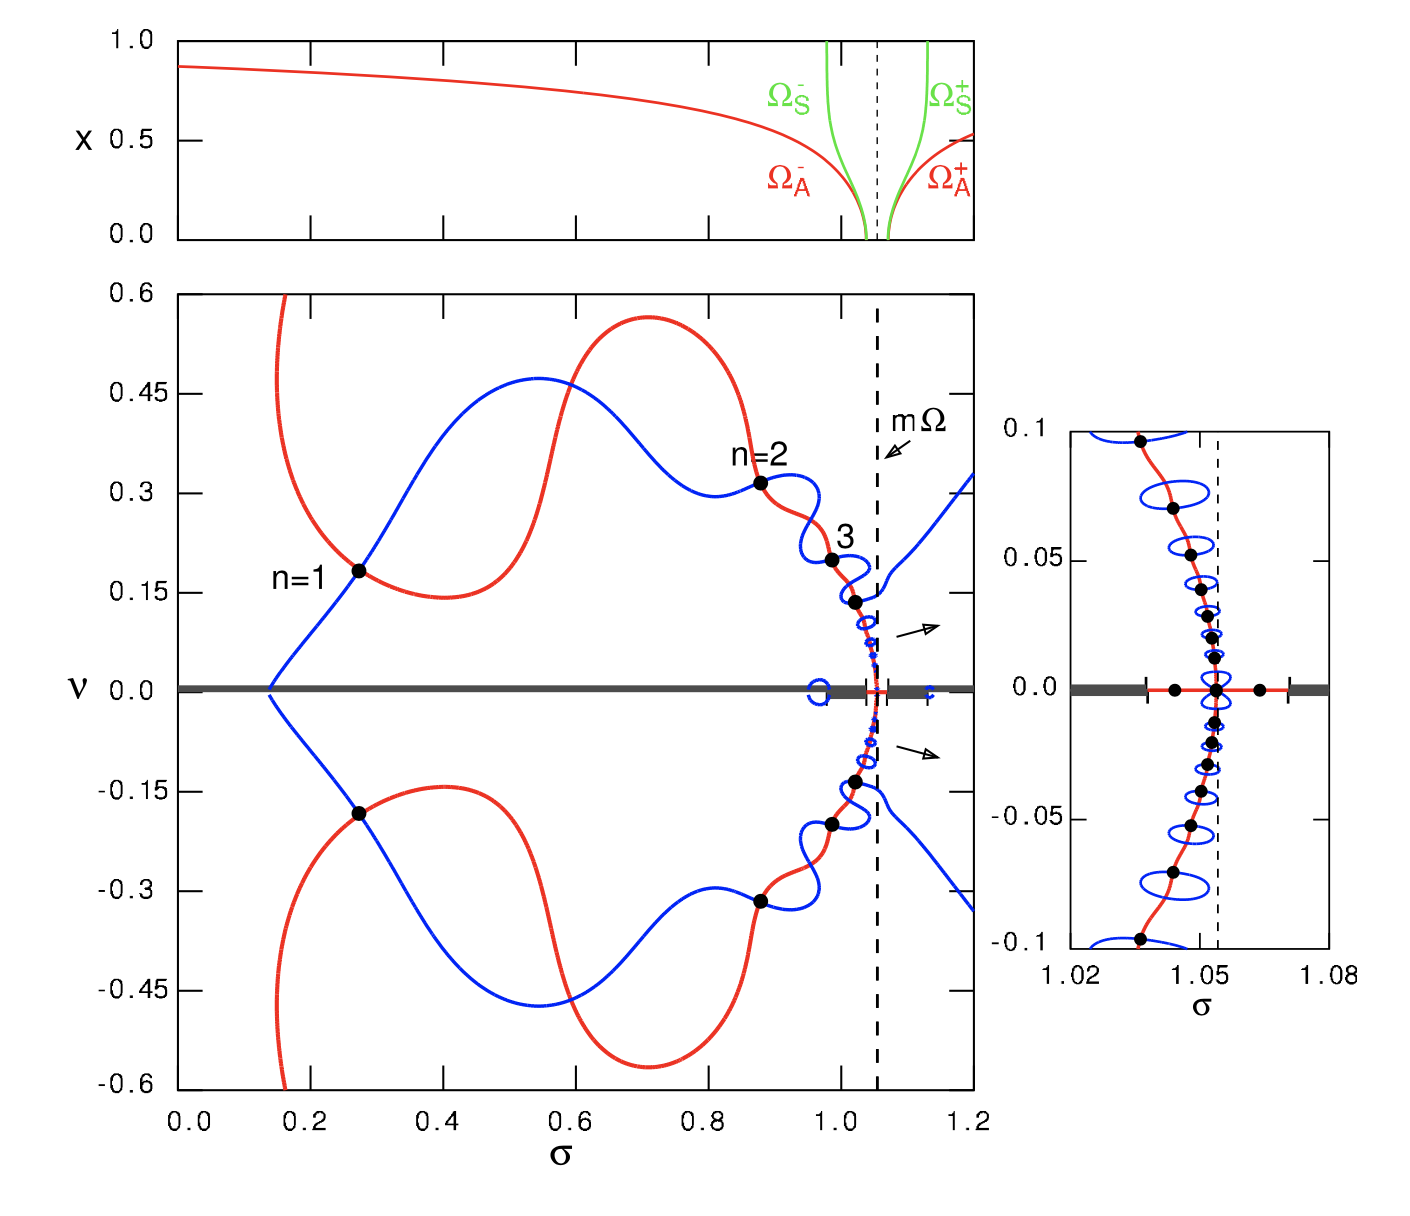
\includegraphics[width=\textwidth]{RTI_MHD.png}
\caption{Values $\rho_0 = a = m = 1$, $\alpha = 2$, $\delta = 1/6$, $k = 0.1$ (magnetohydrodynamics), incompressible.}
	\end{minipage}
\end{figure}

\newpage
\subsection{Magneto-rotational instabilities in accretion disks}
This setup is taken from \citet{goedbloed2018} and models magneto-rotational instabilities in accretion disks. Legolas can model an accretion disk by assuming a cylindrical geometry and letting the grid start from a non-zero value, that is, $r \in [r_0, R]$.
In what follows the parameter $\delta$ denotes $R / r_0$. The equilibrium is given by
\begin{equation*}
	\begin{aligned}[t]
		\rho(r) &= r^{-3/2} \\
		p(r) &= p_1r^{-5/2} \\
		v_\theta(r) &= \Omega_1 r^{-1/2} \\
		B_\theta(r) &= B_{\theta 1}r^{-5/4} \\
		B_z(r) &= B_{z1}r^{-5/4} \\
		g(r) &= \frac{1}{r^2}
	\end{aligned}
	\qquad\qquad
	\begin{aligned}[t]
		\rho'(r) &= -\frac{3}{2}r^{-5/2} \\
		p'(r) &= -\frac{5}{2}p_1 r^{-7/2} \\
		v_\theta'(r) &= -\frac{1}{2}\Omega_1 r^{-3/2} \\
		B_\theta'(r) &= -\frac{5}{4}B_{\theta 1}r^{-9/4} \\
		B_z'(r) &= -\frac{5}{4}B_{z1}r^{-9/4}
	\end{aligned}
\end{equation*}
where
\[ p_1 = \epsilon^2, \qquad B_{z1} = \sqrt{\frac{2p_1}{\beta(1 + \mu_1^2)}}, \qquad B_{\theta 1} = \mu_1 B_{z1}, \qquad v_{\theta 1} = \sqrt{1 - \frac{5}{2}p_1 - \frac{1}{4}B_{\theta 1}^2 - \frac{5}{4}B_{z1}^2} \]

\begin{figure}[h]
	\centering
	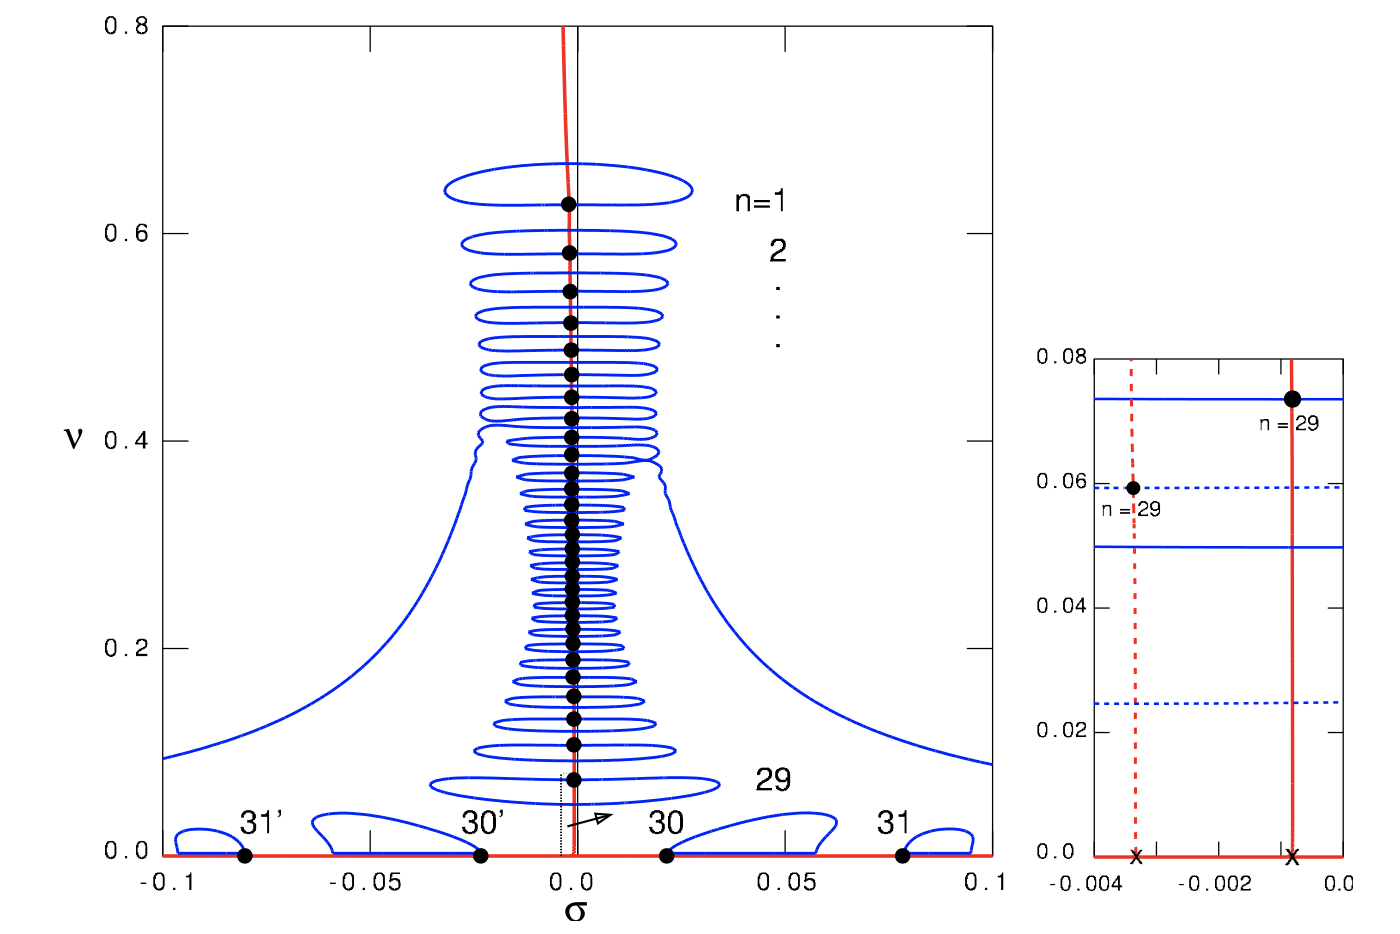
\includegraphics[width=0.8\textwidth]{accretion_disk.png}
	\caption{Values $m = 0$, $k = 70$, $\beta = 100$, $\mu_1 = 1$, $\epsilon = 0.1$ and $\delta = 2$.}
\end{figure}
\bibliographystyle{bibstyle}
\bibliography{bibfile}


\end{document}